\documentclass[a4paper]{article}
\usepackage[utf8]{inputenc}
\usepackage[T1]{fontenc}
\usepackage[pdftex]{graphicx}
\usepackage{fancyhdr}
\usepackage{lscape}
\usepackage{color}
\usepackage{qtree}
\usepackage[english]{babel}
\usepackage{graphicx}
\usepackage[colorinlistoftodos]{todonotes}
\usepackage{listings}
\usepackage{color}
\usepackage{float}
\usepackage{changepage}
\usepackage[margin=1in]{geometry}
\definecolor{codegreen}{rgb}{0,0.6,0}
\definecolor{codegray}{rgb}{0.5,0.5,0.5}
\definecolor{codepurple}{rgb}{0.58,0,0.82}
\definecolor{backcolour}{rgb}{0.95,0.95,0.92}
\usepackage[final]{pdfpages} 
\usepackage[parfill]{parskip}

 
 \lstdefinestyle{mystyle}{
 	backgroundcolor=\color{backcolour},   
 	commentstyle=\color{codegreen},
 	keywordstyle=\color{magenta},
 	numberstyle=\tiny\color{codegray},
 	stringstyle=\color{codepurple},
 	basicstyle=\footnotesize,
 	breakatwhitespace=false,         
 	breaklines=true,                 
 	captionpos=b,                    
 	keepspaces=true,                 
 	numbers=left,                    
 	numbersep=5pt,                  
 	showspaces=false,                
 	showstringspaces=false,
 	showtabs=false,                  
 	tabsize=2
 }
 
\lstset{
	style=mystyle,
	inputencoding=utf8,
	extendedchars=true,
	literate={á}{{\'a}}1 {ã}{{\~a}}1 {é}{{\'e}}1,
	escapechar=\&
}
\title{Algorithmique et structures de données : Mission 4 correction croisée}
\date{14 novembre 2014}
\author{Groupe 1.2: Ivan Ahad - Jérôme Bertaux - Rodolphe Cambier \\ 
	Baptiste Degryse - Wojciech Grynczel - Charles Jaquet}

\begin{document}
\maketitle


Rapport écrit par Rodolphe Cambier, Ivan Ahad et Charles Jaquet.

\section*{Introduction}

A la suite de la mission précédente où l'objectif était de faire un programme permettant d'accéder au classement d'une revue scientifique, cette mission-ci consiste en l'implémentation d'un dictionnaire ordonné,  étant donné qu'on doit pouvoir avoir une liste de ces revues dans l'ordre alphabétique.


\section*{Fonctionnement}

Notre code de la mission précédente permettait déjà la création d'un dictionnaire ordonné, cette mission-ci reprend le même code en rajoutant une interface graphique ainsi qu'un moyen de retourner le dictionnaire trié.


Pour la partie graphique, les classes \textit{Fenetre} et \textit{EntreePanel} sont rajoutées.


Pour trier le dictionnaire, la classe \textit{EntreeComparable} est rajoutée. Ainsi que la fonction \textit{List<Entree> getSortedList()}, utilisée afin de trier la Map contenant les journeaux.


La classe \textit{Performance} est ajoutée pour de réaliser un test de performance.

Le code fonctionne comme suit:

\begin{itemize}
\item La classe \textbf{Main} crée un \textbf{Dictionnaire}.
\item Le \textbf{Dictionnaire} lit le fichier, met chaque ligne sous forme clé-valeur dans une \textbf{Map} ordonnée, en le récupérant de la mission précédente. 
\item La classe \textbf{Main} crée une \textbf{Fenetre}
\item La \textbf{Fenetre} demande une fieldName et fieldValue (Catégorie à rechercher, et String à rechercher dans cette catégorie) ainsi qu'un champ orderBy (Catégorie selon laquelle trier les résultats)
\item La \textbf{Fenetre} va print les résultats après avoir utilisé \textit{getSortedList()} sur le dictionnaire.
\end{itemize}




\section*{Tests réalisés}

La classe \textit{DictionnaireTest} est utilisée afin de tester le programme.

Plusieurs fonctions testent différentes partie du programme, et les différentes limites de celui-ci. 

\section*{Questions par rapport au programme}

\subsubsection*{Question 9(Charles) - Performance}

Pour analyser les performances du tri, j'ai dû modifier le programme pour lui permettre de faire des dictionnaires avec un nombre d'éléments prédéfini. Ensuite j'ai fait les calculs du temps moyens pour créer une liste triée des éléments. Enfin j'ai écris ces temps dans un fichier qui m'a permet de tracer le graphe (fig. \ref{perfo}) du temps nécéssaire pour créer une liste ordonnée en partant de la treeMap en fonction du nombre d'éléments.


\begin{figure} [H]
\begin{center}
\includegraphics[scale=0.4]{performanceListeOrdonnee.eps}
\caption{Graphe du temps pour créer une liste ordonnée en partant du TreeMap en fonction du nombre d'éléments}
\label{perfo}
\end{center}
\end{figure}

Ensuite, en fonction du nombre d'éléments, nous avons calculé le temps pris pour trouver un élément dans la liste. (Fig. \ref{perfoFind})

\begin{figure} [H]
\begin{center}
\includegraphics[scale=0.4]{performanceFind.eps}
\caption{Temps moyen mis pour trouvé un élément}
\label{perfoFind}
\end{center}
\end{figure}

Etonnement, nous avons un temps stable or que nous nous attendions à ce que ça évolue de manière logarithmique

\subsubsection*{Question 10}

Toute la partie de création d'une \textbf{Map} à partir du fichier texte a pu être réutilisée.

 Il a fallut implémenter un système de tri, et donc rajouter les classes comme décrit dans la partie \textbf{Fonctionnement}. Nous avons également choisi d'implémenter une interface graphique.


Le code est plus générique, car il permet de trier dans l'ordre voulu et de choisir le fichier source. La lecture et l'écriture du fichier se fait maintenant dans une classe à part, afin de rendre le fichier plus modulable.

\subsubsection*{Question 11}


\subsection*{Schéma UML}
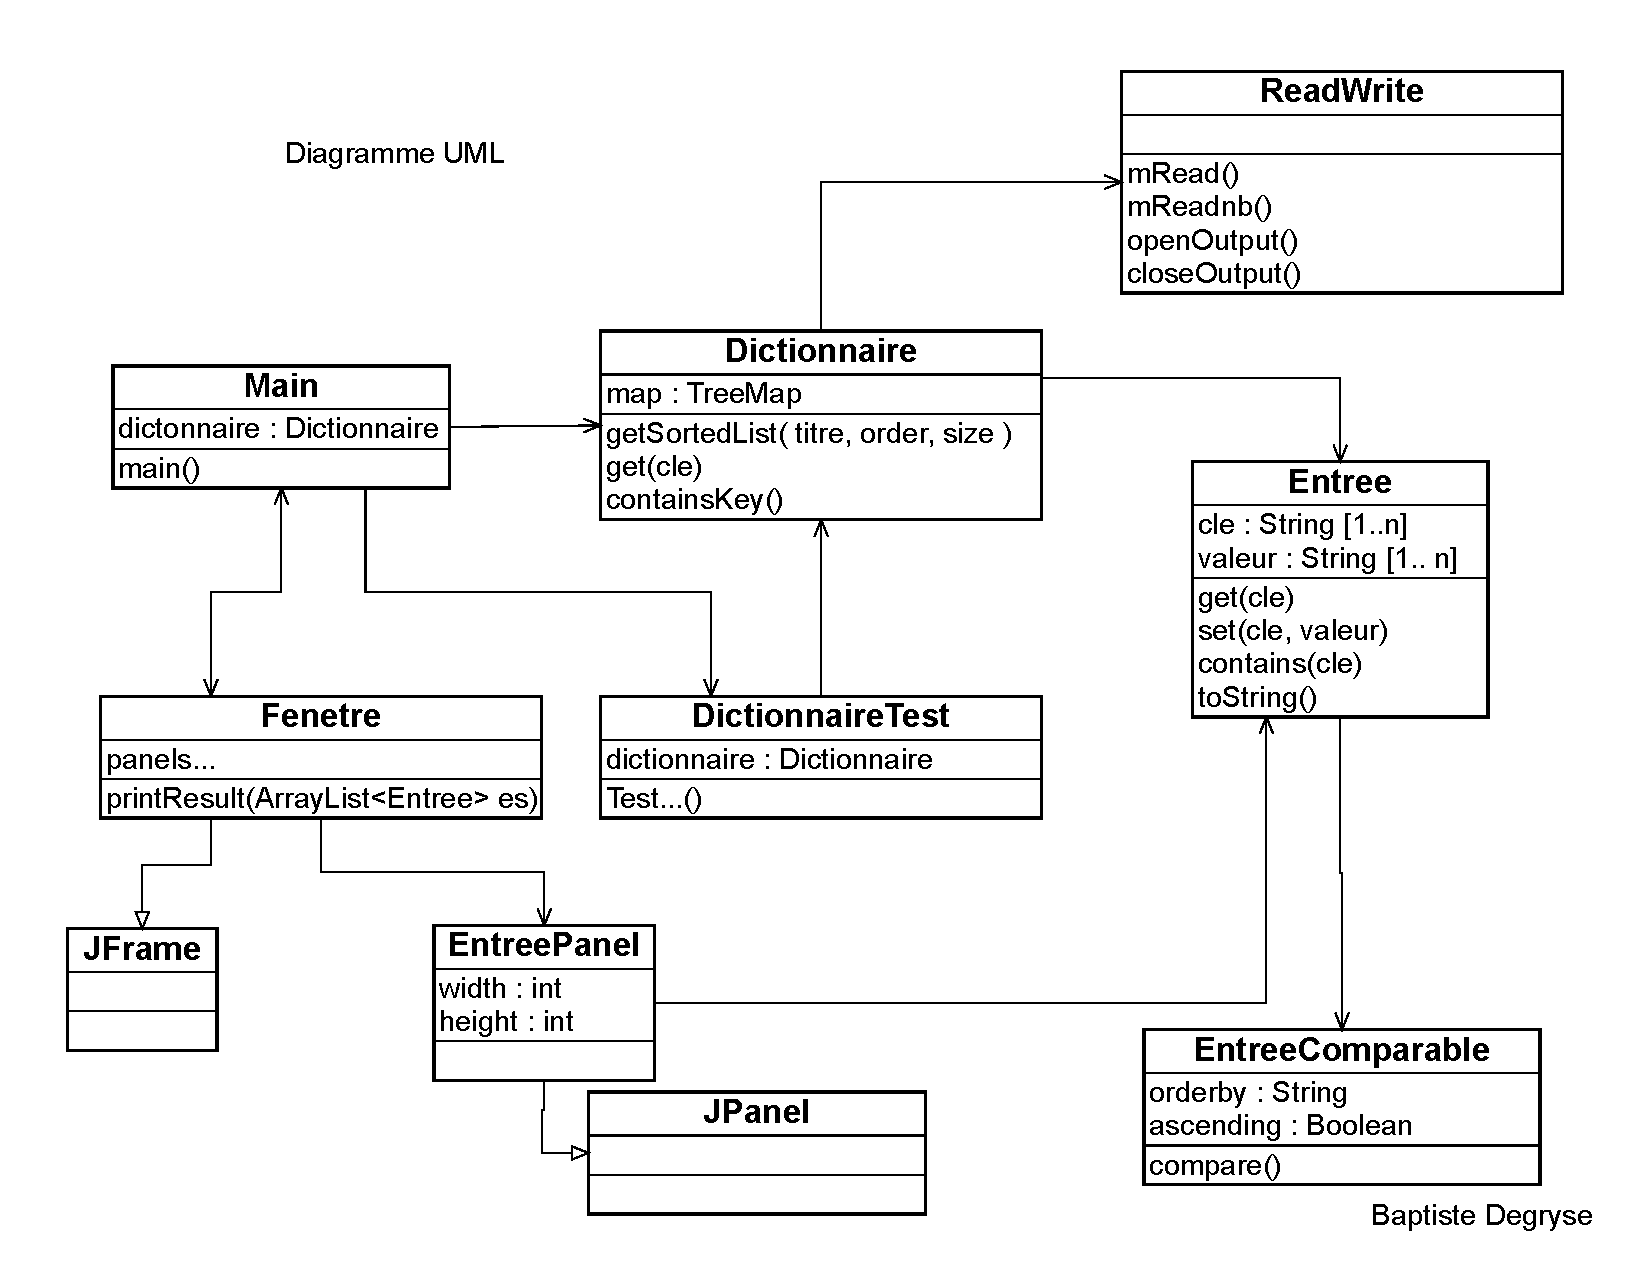
\includegraphics[scale=0.5]{DiagrammeUML.pdf}

\end{document}
